% Figura: um PRB em um slot, com os 4 símbolos de DM-RS (2, 3, 10, 11): 48 REs.
%   Separada da Figura fig:dmrs-n em 2026-11-04 (antes era a parte (a)).
%   Cores: azul da escala do mapa (#cde2fb claro, #0d366b escuro); sem verde; sem negrito.
\definecolor{dmrsfill}{HTML}{CDE2FB}
\definecolor{winblue}{HTML}{0D366B}
\definecolor{inksec}{HTML}{52514E}
\begin{figure}[htbp]
\caption{Resource elements of one PRB in one slot, with the DM-RS symbols.}
\label{fig:prb-dmrs}
\vspace{4pt} % a classe zera o espaço entre a caption e a figura
\centering
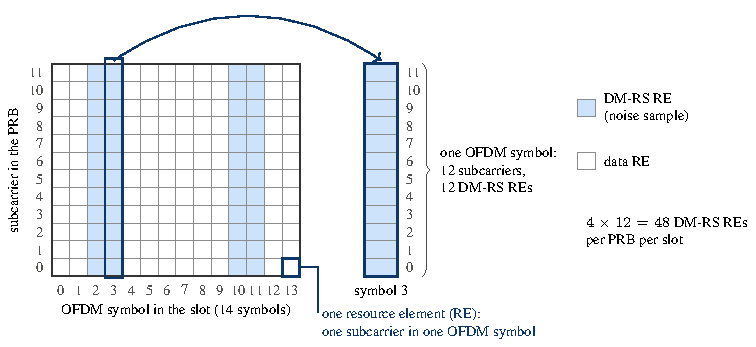
\includegraphics{Images/FLUXO/prb_dmrs.pdf}
\vspace{4pt}
\legend{Source: the author, with the DM-RS positions of \citesp{3gpp-ts38211}. \textcolor{red}{Double-symbol DM-RS}, mapping type~A, symbols 2, 3, 10 and 11.}
\end{figure}
